\subsection{Overview: High level components and their interaction}
The system is divided into three main layers: presentation layer, application layer and data layer. The presentation layer is the interface between the user and the system. It is responsible for the presentation of the data and the interaction with the user. The application layer is the core of the CKB Platform. It is responsible for the business logic and the communication between the presentation layer and the data layer. The data layer is responsible for the storage of the data. It is the interface between the application layer and the database.
\begin{figure}[H]
    \centering
    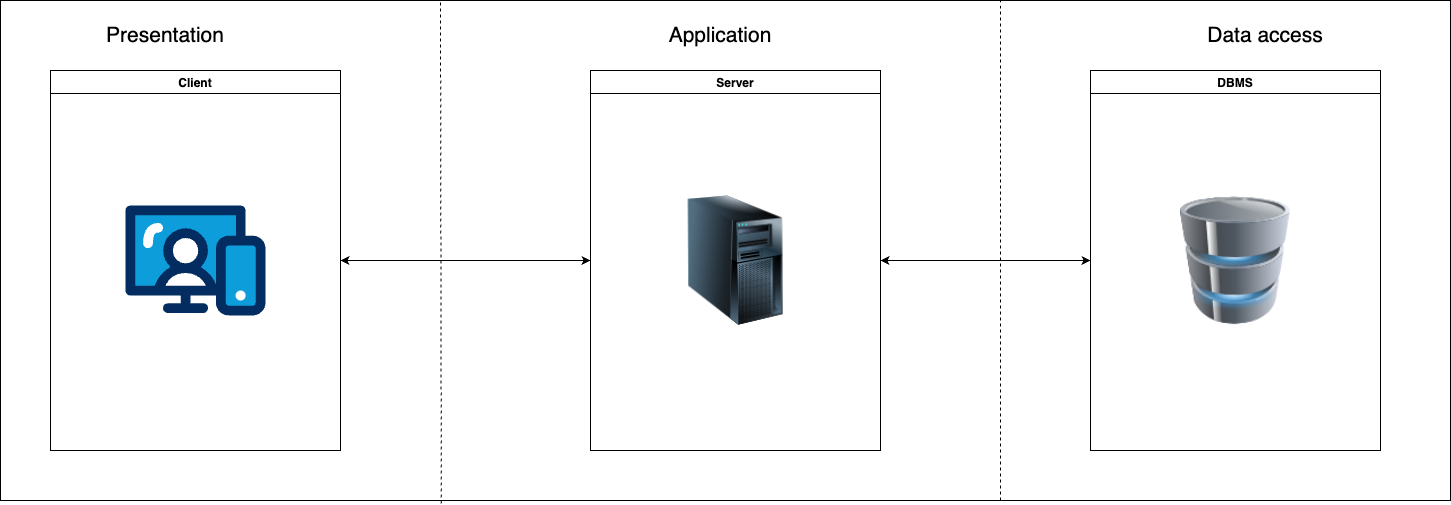
\includegraphics[width=\textwidth]{Images/three_tier.png}
    \caption{High level components and their interaction}
\end{figure}

The three-tier architecture was chosen for this type of system because of the several advantages it offers compared to other types of architectures. For that concerns scalability, it allows for easy scalability by separating the presentation, application, and data layers. Each layer can be scaled independently, allowing for better performance and resource utilization.
For what concers modulatiry, it promotes the separation of concers by dividing the system into distinct layers. This makes it easier to develop, test, and maintain each layer separately, improving overall code quality and reusability. The sepatarion of concerns also improves the maintainability of the system by providing clear boundaries between layers it makes easier to understand and modify specific parts of the system without affecting other layers.
The last advantage for which this architecture was chosen is flexibility. The three-tier provides flexibility in terms of technology choices. Each layer can be implemented using different technologies, allowing for the use of the most suitable tools and frameworks for each specific layer.

\begin{figure}[H]
    \centering
    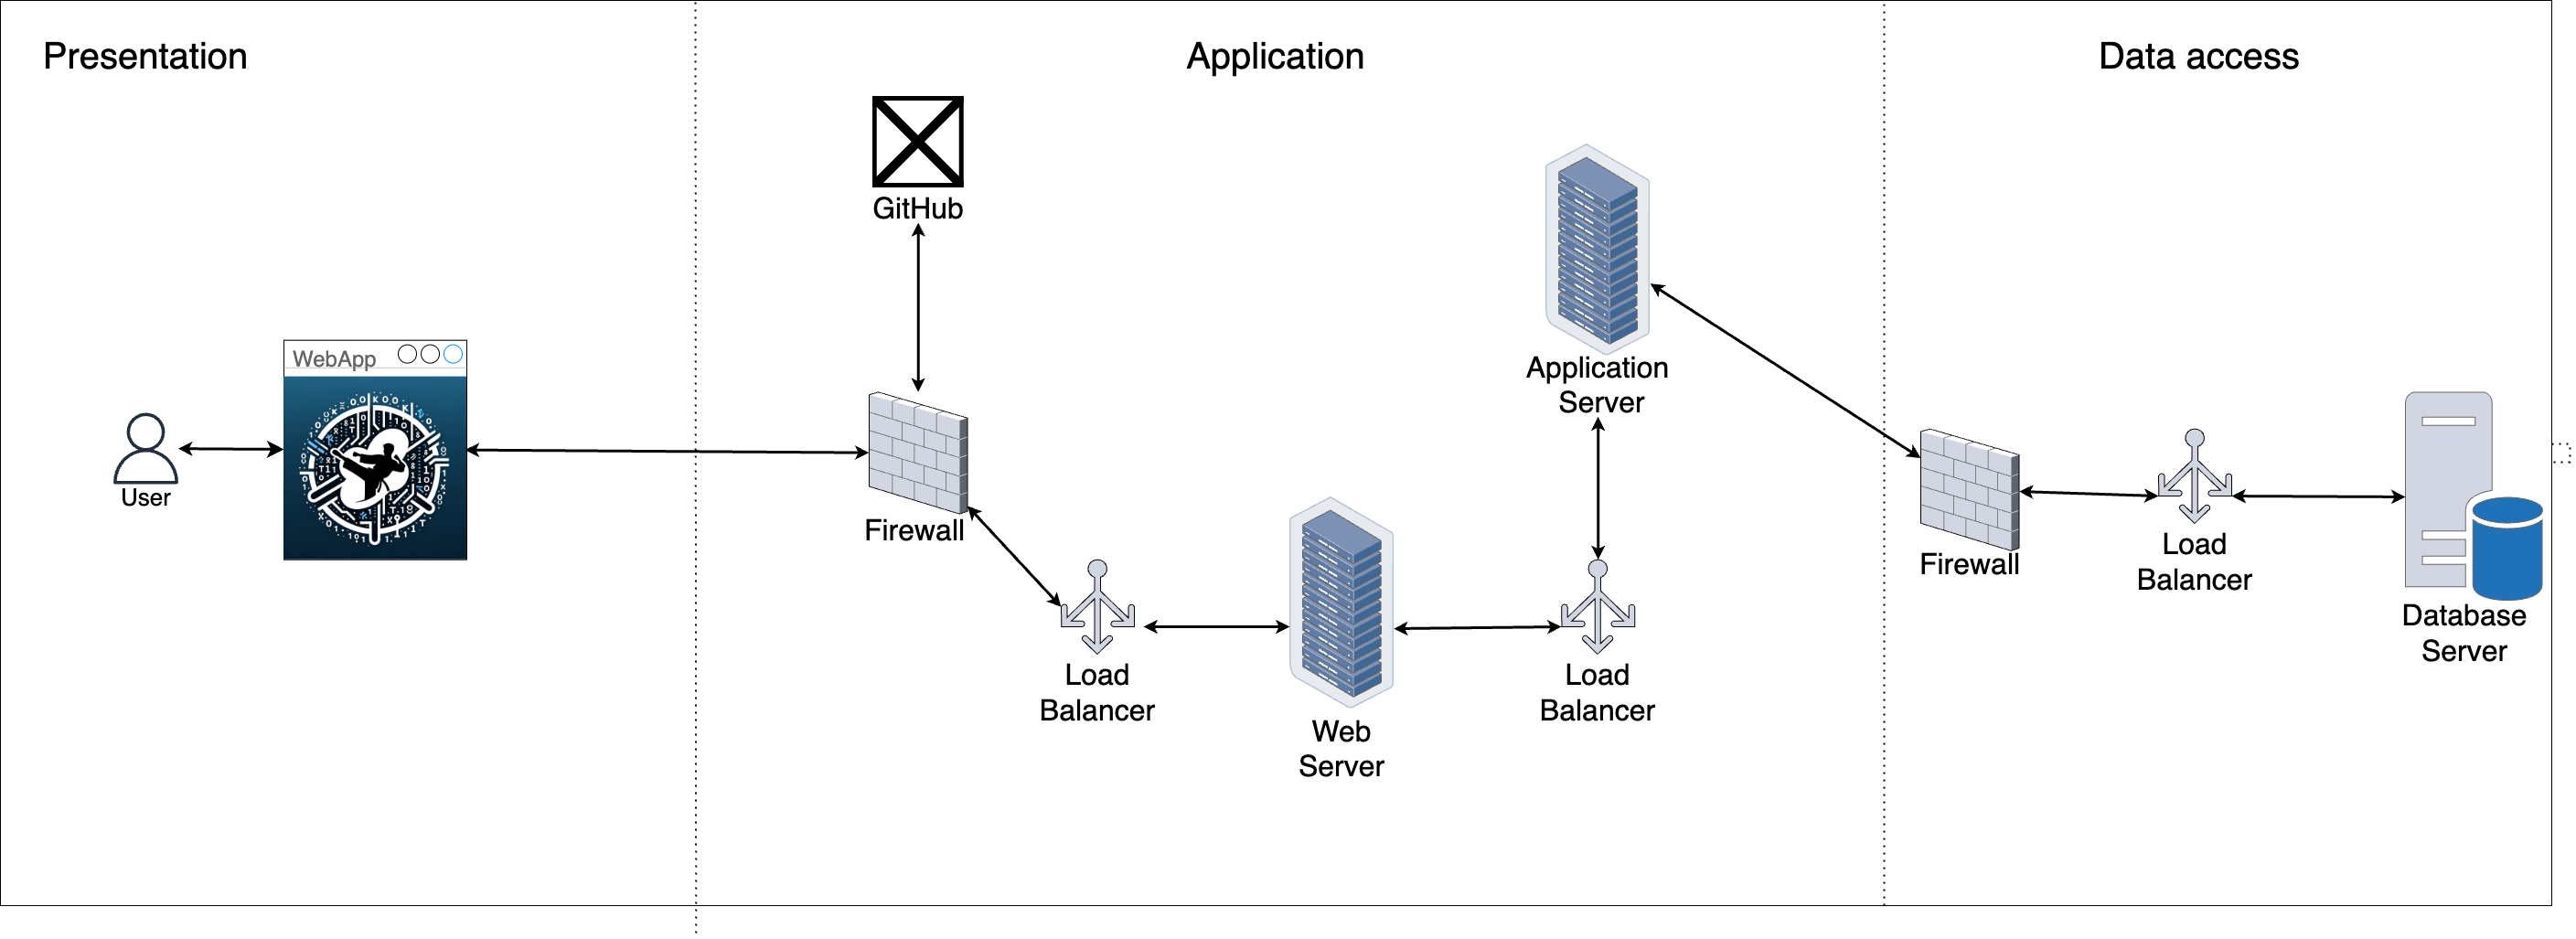
\includegraphics[width=\textwidth]{Images/high_level.png}
    \caption{High level system with interactions between the components}
    \label{fig:high_level_system}
\end{figure}

In the figure Figure\ \ref{fig:high_level_system} is shown the high level system with the interactions between the components. 
At the forefront is the Presentation layer, where a user engages with the web application through a web browser.
The web application depending on user interactions requests data from the web server. The interaction between the two is not direct since there is a firewall (for security reasons) and also a load balancer.

Moving inward, the Application layer serves as the system's operational core, where a network firewall establishes the first line of defense, safeguarding the internal processes. A load balancer stands right behind the firewall, directing incoming traffic to maintain system efficiency and reliability. This layer is further composed by an application server that executes the business logic, interfacing with databases or other external services as needed. Additionally, the presence of an upward arrow connecting the load balancer to GitHub to handle the evaluation trigger as well as the creation of the repositories. This is a very important feature of the system since it allows to automatically evaluate the students' submissions.

The final segment of the diagram is the Data Access layer, echoing the security and balance themes with its own firewall and load balancer, underscoring the system's commitment to secure data transactions. At the heart of this layer lies the database server, a robust storage solution that ensures data is efficiently stored, retrieved, and managed, completing the architecture's promise of a secure, scalable, and resilient web application environment.

\subsection{Component view}
\subsection{Deployment view}
\subsection{Component interfaces}
\subsection{Runtime view}
\subsection{Selected architectural styles and patterns}
\subsection{Other design decisions}
